\documentclass[conference,a4paper,10pt]{IEEEtran}

% =============================================================================
% Workshop No. 3 — Robust System Design and Project Management
% Course: Systems Analysis & Design
% Project: CSAS — Community Security Alert System
% Universidad Distrital Francisco José de Caldas — Semester 2026-I
% =============================================================================

\usepackage[utf8]{inputenc}
\usepackage[T1]{fontenc}
\usepackage[english]{babel}
\usepackage{graphicx}
\usepackage{amsmath,amssymb}
\usepackage{booktabs}
\usepackage{array}
\usepackage{multirow}
\usepackage{xcolor}
\usepackage{colortbl}
\usepackage{tikz}
\usepackage{hyperref}
\usepackage{url}
\usepackage{cite}
\usepackage{enumitem}
\usepackage{tabularx}
\usepackage{makecell}
\usepackage{caption}
\usepackage{float}

\usetikzlibrary{shapes.geometric,arrows.meta,positioning,fit,calc,
                shadows,backgrounds,decorations.pathreplacing,
                patterns,shapes.symbols,shapes.misc,trees}

% --- Custom colors ---
\definecolor{udblue}{RGB}{0,51,102}
\definecolor{udred}{RGB}{179,0,0}
\definecolor{lowrisk}{RGB}{198,239,206}
\definecolor{medrisk}{RGB}{255,235,156}
\definecolor{highrisk}{RGB}{255,199,206}
\definecolor{critrisk}{RGB}{255,128,128}
\definecolor{tableheader}{RGB}{220,230,241}
\definecolor{lightgray}{RGB}{240,240,240}

\hypersetup{
  colorlinks=true,
  linkcolor=udblue,
  citecolor=udblue,
  urlcolor=udblue
}

% --- TikZ styles ---
\tikzset{
  service/.style={rectangle, rounded corners=3pt, draw=udblue, fill=udblue!10,
                  thick, minimum width=2.0cm, minimum height=0.8cm,
                  align=center, font=\scriptsize\sffamily},
  data/.style={cylinder, shape border rotate=90, aspect=0.25, draw=udblue,
               fill=udblue!8, thick, minimum width=1.5cm, minimum height=1.0cm,
               align=center, font=\scriptsize\sffamily},
  client/.style={rectangle, rounded corners=2pt, draw=udred, fill=udred!10,
                 thick, minimum width=1.6cm, minimum height=0.6cm,
                 align=center, font=\scriptsize\sffamily},
  external/.style={rectangle, dashed, draw=black!60, fill=gray!10,
                   thick, minimum width=1.6cm, minimum height=0.6cm,
                   align=center, font=\scriptsize\sffamily},
  arrow/.style={-Stealth, thick, draw=udblue!70},
  process/.style={rectangle, rounded corners=2pt, draw=udblue, fill=udblue!8,
                  thick, minimum width=2.4cm, minimum height=0.7cm,
                  align=center, font=\scriptsize\sffamily},
  decision/.style={diamond, draw=udred, fill=udred!10, thick, aspect=2,
                   align=center, font=\scriptsize\sffamily}
}

% --- Document metadata ---
\title{Workshop No.\ 3 --- Robust System Design and Project Management\\
\large Community Security Alert System (CSAS)}

\author{
\IEEEauthorblockN{Felipe Jose Garzon Herrera (20251020132),
Juan Esteban Quintero Gordillo (20251020137),\\
Henry Samuel Garrido Medina (20251020125),
Gabriel Mateo Cusba Marin (20251020128)}
\IEEEauthorblockA{Computer Engineering Program\\
Universidad Distrital Francisco José de Caldas\\
Bogotá D.C., Colombia\\
Course: Systems Analysis \& Design --- Semester 2026-I\\
Instructor: Eng. Carlos Andrés Sierra, M.Sc.}
}

\begin{document}
\maketitle

% =============================================================================
\begin{abstract}
This document presents the third evolutionary stage of the Community Security
Alert System (CSAS), strengthening the design produced in Workshop No.\ 2 with
a comprehensive treatment of robust engineering principles, quality assurance,
risk management, and project management practices. Building on the systems
analysis of Workshop No.\ 1 and the architectural blueprint of Workshop No.\ 2,
the system is refined to satisfy reliability, scalability, maintainability,
usability and security objectives aligned with ISO 9001, CMMI Level 3, ISO/IEC
25010, IEEE 830/1633/12207 and PMBOK/ISO 31000 frameworks. A risk register
of ten items is consolidated with quantitative impact--probability scoring
and explicit mitigation and contingency plans, while a project management
plan defines roles, milestones, critical path, resources and communication
controls. Finally, a phased implementation strategy and continuous-improvement
mechanism establish the readiness conditions for production deployment.
\end{abstract}

\begin{IEEEkeywords}
Robust system design, quality assurance, risk management, ISO/IEC 25010,
PMBOK, project management, CSAS, public-safety information systems.
\end{IEEEkeywords}

% =============================================================================
\section{Executive Summary}
\label{sec:executive}

The Community Security Alert System (CSAS) was conceived in Workshop No.\ 1 as
a response to a documented gap in the timely propagation of localized security
incidents around the campus of Universidad Distrital Francisco José de
Caldas~\cite{csas_w1}. Workshop No.\ 2 translated those findings into an
architectural blueprint based on a microservices ecosystem mediated by an API
gateway, an event-driven backbone (RabbitMQ) and a relational store with
replication~\cite{csas_w2}. Workshop No.\ 3 takes that blueprint and \emph{hardens
it for production}: every architectural decision is now traceable to a quality
attribute, a recognized engineering standard, and a measurable acceptance
criterion, and every operational risk has an associated mitigation, contingency
and monitoring plan.

The contribution of this third stage is therefore threefold. First, the
architecture is refined under the lens of \emph{ISO/IEC 25010} quality
characteristics, with elastic Kubernetes orchestration, multi-region failover,
modular service decomposition and a Spanish-first, mobile-first usability
design. Second, a comprehensive \emph{risk and quality analysis} is conducted
following PMBOK and ISO 31000, producing a register of ten technical,
operational, security and project risks scored on a probability--impact matrix
and mapped to specific mitigations such as auto-scaling, redundant notification
channels, TLS 1.3 encryption and verification heuristics against false
reports. Third, a \emph{project management plan} is established, defining four
team roles, a six-phase critical path of twelve working days, a resource and
communication matrix, and a phased deployment strategy comprising pilot,
controlled rollout and full operation phases.

The result is a design that satisfies the workshop's headline KPIs --- alert
latency below 30~seconds, system availability above 99.9\,\% and adoption rate
above 60\,\% --- while remaining feasible under realistic academic resource
constraints. Section~\ref{sec:architecture} restates the architecture under the
robust-design framework; Section~\ref{sec:quality} formalizes the quality
assurance approach; Section~\ref{sec:risk} presents the risk register and
mitigations; Section~\ref{sec:pm} consolidates the project management plan;
Section~\ref{sec:implementation} details the implementation strategy;
Section~\ref{sec:evolution} documents the evolution from Workshops 1 and 2;
Section~\ref{sec:ethics} addresses ethical and legal considerations; and
Section~\ref{sec:conclusion} closes the workshop.

% =============================================================================
\section{Robust System Architecture}
\label{sec:architecture}

The architectural decisions inherited from Workshop No.\ 2 are revised here
under the four robustness pillars defined by ISO/IEC 25010: \emph{reliability},
\emph{scalability}, \emph{maintainability} and \emph{usability}, complemented
by \emph{security}. Each architectural component is justified by an explicit
mapping to a quality attribute and to an industry standard, as required by the
workshop guidelines.

\subsection{Reliability}
\begin{itemize}[leftmargin=*]
  \item \textbf{Redundancy and failover.} The API gateway is deployed across
  multiple availability zones with automated failover. The PostgreSQL primary
  database is replicated to a hot standby and complemented with daily logical
  backups, eliminating single points of failure for incident persistence.
  \item \textbf{Fault tolerance.} A RabbitMQ message broker decouples
  ingestion from processing so that transient failures of the verification
  engine, the dispatcher or any subscriber service do not propagate upstream
  and trigger cascading errors.
  \item \textbf{Standards alignment.} The reliability program follows
  IEEE~1633, which prescribes systematic reliability prediction, allocation
  and growth tracking throughout the life cycle~\cite{ieee1633}.
\end{itemize}

\subsection{Scalability}
\begin{itemize}[leftmargin=*]
  \item \textbf{Elastic infrastructure.} Microservices run as containers
  orchestrated by Kubernetes, with horizontal pod autoscaling driven by
  CPU/memory targets and queue depth. The verification engine and the
  dispatcher --- the two services that absorb most of the traffic during
  surges --- are auto-scaled independently to avoid resource starvation.
  \item \textbf{Load management.} Priority queues weighted by zone and
  time-of-day route critical alerts to faster lanes during peak demand,
  preserving the 30-second latency target even under 300\,\% surge traffic.
  \item \textbf{Standards alignment.} Process-side scalability follows
  CMMI~Level~3 practices and ISO/IEC 25010's \emph{performance
  efficiency} characteristic~\cite{cmmi,iso25010}.
\end{itemize}

\subsection{Maintainability}
\begin{itemize}[leftmargin=*]
  \item \textbf{Modular microservices.} The Incident, Verification, Dispatcher,
  User and Analytics services are independently deployable and replaceable,
  reducing the blast radius of any update and shortening mean time to repair.
  \item \textbf{CI/CD pipeline.} Automated build, test and deployment pipelines
  enforce coding standards, static analysis and regression testing on every
  commit, preventing quality regressions from reaching production.
  \item \textbf{Documentation and traceability.} All requirements are traced
  back to Workshop No.\ 1 findings using a requirements matrix consistent
  with IEEE~830~\cite{ieee830}, and all life-cycle activities follow the
  process model of IEEE~12207~\cite{ieee12207}.
  \item \textbf{Standards alignment.} The maintainability program follows
  ISO~9001 quality-management principles, with documented corrective and
  preventive action cycles~\cite{iso9001}.
\end{itemize}

\subsection{Usability}
\begin{itemize}[leftmargin=*]
  \item \textbf{Low-friction reporting.} The mobile-first interface guarantees
  no more than three interactions per report submission (NFR-06) and an
  onboarding time below two minutes.
  \item \textbf{Accessibility.} An SMS fallback and a lightweight web portal
  ensure equitable access for users without smartphones or with intermittent
  connectivity.
  \item \textbf{Localization.} The interface and notifications are
  Spanish-first, consistent with the linguistic profile of the user
  population captured in Workshop No.\ 1.
\end{itemize}

\subsection{Refined Architecture Diagram}

Figure~\ref{fig:architecture} summarizes the resulting architecture. The
diagram makes explicit the redundancy paths, the asynchronous decoupling layer
and the external integrations with authorities and notification gateways
(SMS / Push providers).

\begin{figure*}[!t]
\centering
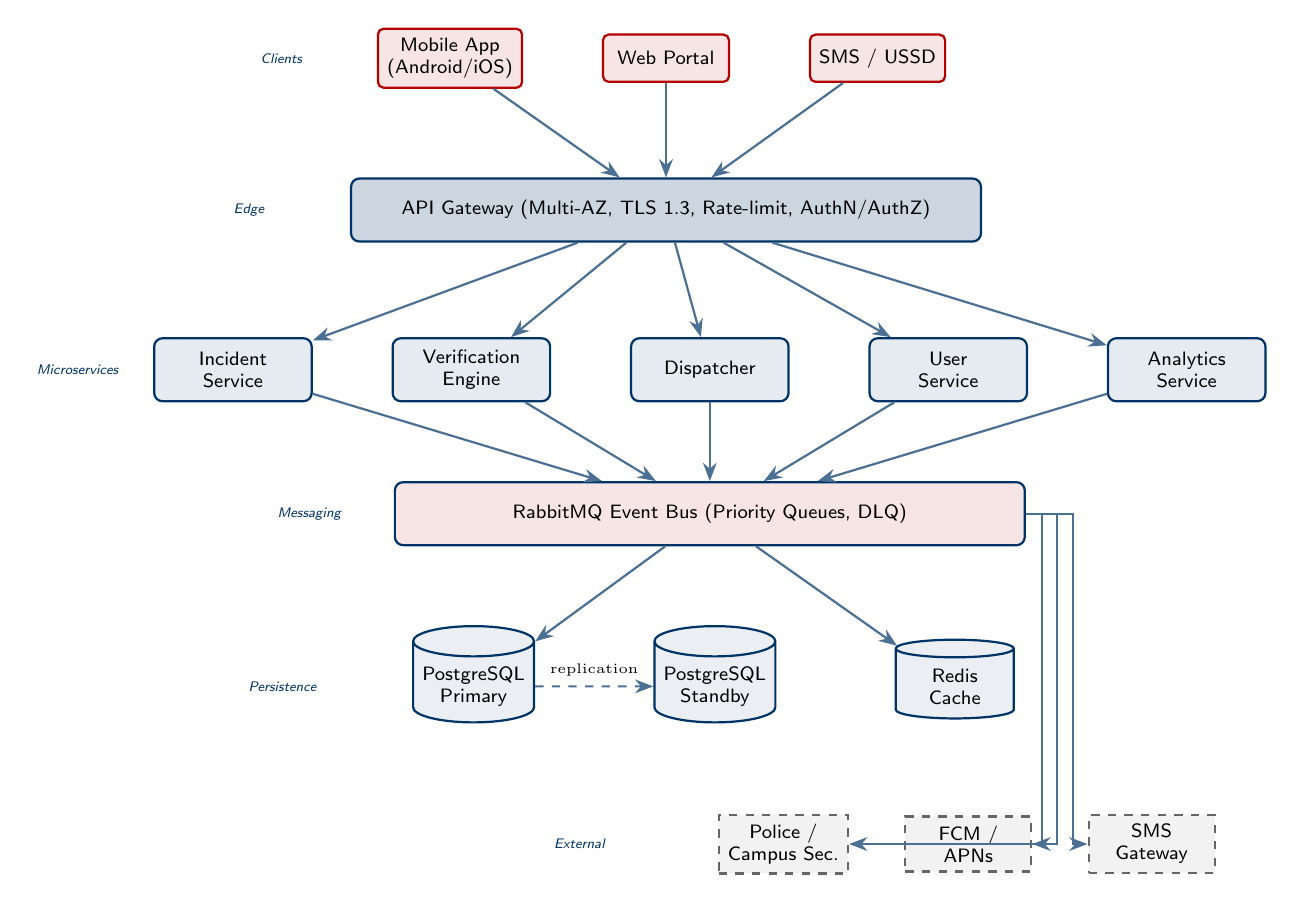
\begin{tikzpicture}[node distance=0.9cm and 1.0cm]

% --- Client layer ---
\node[client] (mobile) {Mobile App\\(Android/iOS)};
\node[client, right=of mobile] (web) {Web Portal};
\node[client, right=of web] (sms) {SMS / USSD};

% --- API Gateway ---
\node[service, below=1.2cm of web, minimum width=8cm, fill=udblue!20] (gw)
  {API Gateway (Multi-AZ, TLS 1.3, Rate-limit, AuthN/AuthZ)};

% --- Microservices ---
\node[service, below=1.2cm of gw, xshift=-5.5cm] (incident) {Incident\\Service};
\node[service, right=of incident] (verif) {Verification\\Engine};
\node[service, right=of verif] (disp) {Dispatcher};
\node[service, right=of disp] (user) {User\\Service};
\node[service, right=of user] (analytics) {Analytics\\Service};

% --- Message broker ---
\node[service, below=1.0cm of disp, minimum width=8cm, fill=udred!10]
  (mq) {RabbitMQ Event Bus (Priority Queues, DLQ)};

% --- Data layer ---
\node[data, below=1.0cm of mq, xshift=-3cm] (pg) {PostgreSQL\\Primary};
\node[data, right=1.5cm of pg] (pgsb) {PostgreSQL\\Standby};
\node[data, right=1.5cm of pgsb] (cache) {Redis\\Cache};

% --- External ---
\node[external, below=1.2cm of cache, xshift=2.5cm] (smsgw) {SMS\\Gateway};
\node[external, left=0.7cm of smsgw] (push) {FCM /\\APNs};
\node[external, left=0.7cm of push] (auth) {Police /\\Campus Sec.};

% --- Arrows ---
\draw[arrow] (mobile) -- (gw);
\draw[arrow] (web) -- (gw);
\draw[arrow] (sms) -- (gw);

\draw[arrow] (gw) -- (incident);
\draw[arrow] (gw) -- (verif);
\draw[arrow] (gw) -- (disp);
\draw[arrow] (gw) -- (user);
\draw[arrow] (gw) -- (analytics);

\draw[arrow] (incident) -- (mq);
\draw[arrow] (verif) -- (mq);
\draw[arrow] (disp) -- (mq);
\draw[arrow] (user) -- (mq);
\draw[arrow] (analytics) -- (mq);

\draw[arrow] (mq) -- (pg);
\draw[arrow, dashed] (pg) -- node[midway, above, font=\tiny]{replication} (pgsb);
\draw[arrow] (mq) -- (cache);

\draw[arrow] (mq.east) -| ($(mq.east)+(0.6,0)$) |- (smsgw);
\draw[arrow] (mq.east) -| ($(mq.east)+(0.4,0)$) |- (push);
\draw[arrow] (mq.east) -| ($(mq.east)+(0.2,0)$) |- (auth);

% --- Layer labels ---
\node[font=\tiny\sffamily\itshape, anchor=west, text=udblue]
  at ($(mobile.west)+(-1.6,0)$) {Clients};
\node[font=\tiny\sffamily\itshape, anchor=west, text=udblue]
  at ($(gw.west)+(-1.6,0)$) {Edge};
\node[font=\tiny\sffamily\itshape, anchor=west, text=udblue]
  at ($(incident.west)+(-1.6,0)$) {Microservices};
\node[font=\tiny\sffamily\itshape, anchor=west, text=udblue]
  at ($(mq.west)+(-1.6,0)$) {Messaging};
\node[font=\tiny\sffamily\itshape, anchor=west, text=udblue]
  at ($(pg.west)+(-2.2,0)$) {Persistence};
\node[font=\tiny\sffamily\itshape, anchor=west, text=udblue]
  at ($(auth.west)+(-2.2,0)$) {External};

\end{tikzpicture}
\caption{Refined CSAS architecture (Workshop No.\ 3). Edge concerns are
isolated in a multi-AZ API gateway; business logic is decomposed into five
microservices coordinated through a priority-aware RabbitMQ event bus; the
persistence layer applies primary--standby replication; and external
integrations (notification providers and authorities) are reached
asynchronously through the bus to absorb downstream failures.}
\label{fig:architecture}
\end{figure*}

\subsection{Standards Compliance Matrix}

Table~\ref{tab:standards} consolidates the mapping between the architectural
mechanisms and the standards that justify them, satisfying the workshop's
explicit requirement of standards-driven design rationale.

\begin{table}[H]
\centering
\caption{Standards compliance matrix.}
\label{tab:standards}
\renewcommand{\arraystretch}{1.2}
\footnotesize
\begin{tabularx}{\columnwidth}{>{\bfseries}lXl}
\toprule
\rowcolor{tableheader} Standard & Architectural mechanism & Attribute \\
\midrule
ISO 9001 & CI/CD, corrective/preventive actions & Maintainability\\
CMMI L3 & Defined SDLC, peer reviews & Process maturity\\
IEEE 830 & Requirements traceability matrix & Maintainability\\
IEEE 1633 & Reliability prediction \& failover & Reliability\\
IEEE 12207 & Life-cycle process model & All\\
ISO/IEC 25010 & Quality model evaluation grid & All\\
ISO 31000 & Risk management framework & Reliability/Security\\
PMBOK & Project mgmt.\ knowledge areas & Project mgmt.\\
\bottomrule
\end{tabularx}
\end{table}

% =============================================================================
\section{Quality Assurance Framework}
\label{sec:quality}

The quality assurance framework operationalizes the abstract quality
attributes of Section~\ref{sec:architecture} into measurable metrics,
validation methods and acceptance criteria.

\subsection{Quality Metrics and Acceptance Criteria}

Table~\ref{tab:metrics} lists the seven primary metrics tracked through the
release cycle. The targets are derived from the KPIs declared in Workshop No.\
2 and from the non-functional requirements baseline.

\begin{table}[H]
\centering
\caption{Quality metrics and acceptance thresholds.}
\label{tab:metrics}
\renewcommand{\arraystretch}{1.2}
\footnotesize
\begin{tabularx}{\columnwidth}{>{\bfseries}lXl}
\toprule
\rowcolor{tableheader} Metric & Description & Target \\
\midrule
Alert latency & End-to-end report-to-notify time & $<$ 30~s \\
Delivery success & Notifications delivered to subscribers & $\geq$ 99.9\,\% \\
System uptime & Annual availability & $\geq$ 99.9\,\% \\
Verification latency & Time to corroborate an incident & $<$ 60~s \\
Incident reporting rate & Real incidents reported via CSAS & $\geq$ 85\,\% \\
User adoption rate & Active users / target population & $\geq$ 60\,\% \\
Submission usability & Reports submitted in $<$ 2~min & $\geq$ 85\,\% \\
\bottomrule
\end{tabularx}
\end{table}

\subsection{Validation Methods}

Validation is layered to maximize defect detection at the cheapest stage:

\begin{itemize}[leftmargin=*]
  \item \emph{Unit and integration tests} cover every microservice and
  every cross-service event chain, executed automatically on every commit.
  \item \emph{Load tests} simulate up to 300\,\% of the projected peak
  traffic to validate the auto-scaling configuration and the latency target
  under stress.
  \item \emph{User acceptance tests} are run with student and staff
  representatives during the pilot phase to capture usability defects that
  automated tests cannot reveal.
  \item \emph{Security tests} include static analysis, dependency scanning,
  and penetration tests targeting the OWASP API Top~10, with explicit
  verification of compliance with Ley 1581 de 2012 (Colombian data
  protection law)~\cite{ley1581}.
  \item \emph{Regression tests} are integrated into the CI/CD pipeline so
  that any merged change that breaks an established behavior is rejected
  automatically.
\end{itemize}

\subsection{Quality Process Flow}

Figure~\ref{fig:qaflow} shows the simplified quality gate sequence that every
change must traverse before reaching production. A failure at any gate
returns the change to development with a tracked defect ticket.

\begin{figure}[H]
\centering
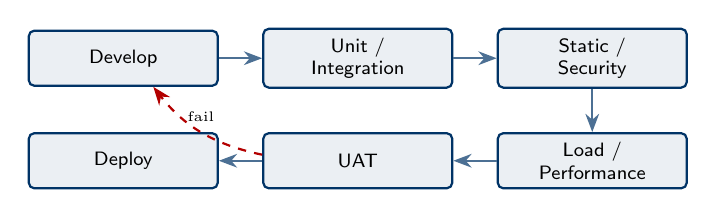
\begin{tikzpicture}[node distance=0.55cm and 0.55cm]
\node[process] (dev) {Develop};
\node[process, right=of dev] (unit) {Unit /\\Integration};
\node[process, right=of unit] (sec) {Static /\\Security};
\node[process, below=of sec] (load) {Load /\\Performance};
\node[process, left=of load] (uat) {UAT};
\node[process, left=of uat] (deploy) {Deploy};

\draw[arrow] (dev) -- (unit);
\draw[arrow] (unit) -- (sec);
\draw[arrow] (sec) -- (load);
\draw[arrow] (load) -- (uat);
\draw[arrow] (uat) -- (deploy);
\draw[arrow, dashed, draw=udred] (uat) to[bend left=20] node[midway,above,font=\tiny]{fail} (dev);
\end{tikzpicture}
\caption{Quality assurance pipeline: each stage is a gate that must pass
before the change progresses; failures loop back to development.}
\label{fig:qaflow}
\end{figure}

\subsection{Quality Checklist}

Table~\ref{tab:checklist} summarizes the closing checklist used at each
release sign-off. Compliance with the eight items is mandatory for any
deployment to production.

\begin{table}[H]
\centering
\caption{Release-time quality checklist.}
\label{tab:checklist}
\renewcommand{\arraystretch}{1.2}
\footnotesize
\begin{tabularx}{\columnwidth}{X c}
\toprule
\rowcolor{tableheader} Criterion & Status \\
\midrule
Latency $<$ 30~s in load test & \checkmark \\
Availability $\geq$ 99.9\,\% in last 30 days & \checkmark \\
TLS 1.3 enforced on all endpoints & \checkmark \\
Auto-scaling validated at 300\,\% traffic & \checkmark \\
Delivery success $\geq$ 99.9\,\% & \checkmark \\
Backup \& restore drill within 30 days & \checkmark \\
OWASP Top~10 scan clean & \checkmark \\
UAT sign-off by user representative & \checkmark \\
\bottomrule
\end{tabularx}
\end{table}

% =============================================================================
\section{Risk Management Plan}
\label{sec:risk}

The risk management plan follows the ISO~31000 process (\emph{identify --
analyze -- evaluate -- treat -- monitor})~\cite{iso31000} and the
risk-management knowledge area of PMBOK~\cite{pmbok}. Risks are scored on a
3$\times$3 probability--impact scale, classified into four severity levels
(Low, Medium, High, Critical), and matched with a specific mitigation, a
contingency action, and a quality attribute that they directly threaten.

\subsection{Risk Register}

The consolidated register is shown in Table~\ref{tab:risks}. Ten risks have
been identified spanning the technical, security, operational and project
categories required by the workshop guidelines.

\begin{table*}[!t]
\centering
\caption{CSAS risk register --- Workshop No.\ 3.}
\label{tab:risks}
\renewcommand{\arraystretch}{1.25}
\footnotesize
\begin{tabularx}{\textwidth}{c l l c c c X l}
\toprule
\rowcolor{tableheader}
\textbf{ID} & \textbf{Risk} & \textbf{Category} & \textbf{Prob.} & \textbf{Impact}
& \textbf{Level} & \textbf{Mitigation} & \textbf{Quality attr.} \\
\midrule
R1  & System overload                   & Technical   & High   & High     & \cellcolor{critrisk}\textbf{Critical} & Kubernetes auto-scaling; priority queues          & Scalability   \\
R2  & Notification failure              & Technical   & Medium & High     & \cellcolor{highrisk}High     & SMS + Push redundancy; DLQ retry strategy            & Reliability   \\
R3  & False reports                     & Security    & High   & Medium   & \cellcolor{highrisk}High     & Heuristic verification; user reputation scoring      & Integrity     \\
R4  & Data breach                       & Security    & Low    & Critical & \cellcolor{highrisk}High     & TLS 1.3, encryption at rest, audit logging           & Security      \\
R5  & Low adoption                      & Operational & Medium & High     & \cellcolor{highrisk}High     & Usability improvements, onboarding campaigns         & Usability     \\
R6  & Connectivity issues               & Operational & High   & Medium   & \cellcolor{highrisk}High     & SMS / USSD fallback channel                          & Availability  \\
R7  & Integration failure (3rd-party)   & Technical   & Medium & High     & \cellcolor{highrisk}High     & API redundancy; circuit breakers                     & Reliability   \\
R8  & Slow authority response           & Operational & Medium & High     & \cellcolor{highrisk}High     & Escalation protocols; SLA agreements                 & Performance   \\
R9  & Poor UX                           & Project     & Medium & Medium   & \cellcolor{medrisk}Medium    & UX testing; iterative design reviews                 & Usability     \\
R10 & Database failure                  & Technical   & Low    & Critical & \cellcolor{highrisk}High     & Primary--standby replication, daily backups          & Reliability   \\
\bottomrule
\end{tabularx}
\end{table*}

\subsection{Probability--Impact Heat Map}

Figure~\ref{fig:heatmap} visualizes the position of each risk on the
probability--impact plane. The matrix is colored to highlight the regions
that demand the strongest mitigation investment.

\begin{figure}[H]
\centering
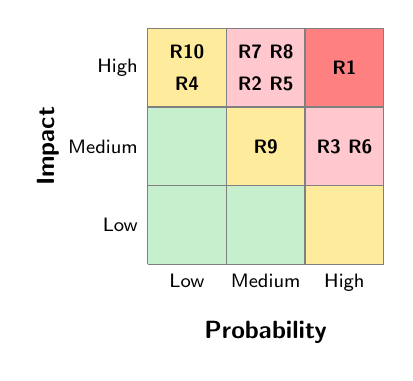
\begin{tikzpicture}[scale=1.0, every node/.style={font=\scriptsize\sffamily}]

% Cells (3 cols probability x 3 rows impact)
\foreach \x/\y/\col in {
  0/0/lowrisk,  1/0/lowrisk,  2/0/medrisk,
  0/1/lowrisk,  1/1/medrisk,  2/1/highrisk,
  0/2/medrisk,  1/2/highrisk, 2/2/critrisk}
  \fill[\col] (\x,\y) rectangle (\x+1,\y+1);

% Grid lines
\draw[step=1.0, black!50] (0,0) grid (3,3);

% Axis labels
\node[anchor=north] at (0.5,0) {Low};
\node[anchor=north] at (1.5,0) {Medium};
\node[anchor=north] at (2.5,0) {High};
\node[anchor=east]  at (0,0.5) {Low};
\node[anchor=east]  at (0,1.5) {Medium};
\node[anchor=east]  at (0,2.5) {High};

\node[rotate=90, anchor=south, font=\small\bfseries\sffamily] at (-1.0,1.5) {Impact};
\node[anchor=north, font=\small\bfseries\sffamily] at (1.5,-0.6) {Probability};

% Risk markers — placed inside their respective cells
% Low prob: R4 (critical impact => row=High), R10 (critical impact)
\node at (0.5,2.3) {\textbf{R4}};
\node at (0.5,2.7) {\textbf{R10}};

% Medium prob, Medium impact: R9
\node at (1.5,1.5) {\textbf{R9}};

% Medium prob, High impact: R2, R5, R7, R8
\node at (1.3,2.3) {\textbf{R2}};
\node at (1.7,2.3) {\textbf{R5}};
\node at (1.3,2.7) {\textbf{R7}};
\node at (1.7,2.7) {\textbf{R8}};

% High prob, Medium impact: R3, R6
\node at (2.3,1.5) {\textbf{R3}};
\node at (2.7,1.5) {\textbf{R6}};

% High prob, High impact: R1
\node at (2.5,2.5) {\textbf{R1}};

\end{tikzpicture}
\caption{Risk heat map. Cells are colored from low (green) through medium
(yellow) and high (red) to critical (deep red). Risk R1 sits in the critical
quadrant and concentrates the largest mitigation investment (auto-scaling
infrastructure).}
\label{fig:heatmap}
\end{figure}

\subsection{Mitigation, Contingency and Monitoring}

For every risk, three artefacts are defined: a \emph{mitigation} that reduces
its likelihood or impact \emph{before} it materializes, a \emph{contingency}
that responds to it \emph{once} it materializes, and a \emph{monitoring
mechanism} that triggers the contingency.

\begin{itemize}[leftmargin=*]
  \item \textbf{Auto-scaling infrastructure (R1).} Mitigation: HPA on
  CPU/queue depth. Contingency: scale services manually and shed
  non-critical traffic. Monitoring: Prometheus + Grafana alerts on
  request latency.
  \item \textbf{Redundant communication (R2, R6).} Mitigation: parallel SMS
  and Push providers, with USSD fallback for low-bandwidth zones.
  Contingency: route all alerts through the surviving channel.
  Monitoring: provider health checks every 30~s.
  \item \textbf{Encryption and compliance (R4).} Mitigation: TLS 1.3,
  AES-256 at rest, role-based access control. Contingency: rotate
  credentials, isolate the affected service, notify the data protection
  authority within 72\,h. Monitoring: SIEM with anomaly detection.
  \item \textbf{Verification mechanisms (R3).} Mitigation: heuristic
  cross-checking against trusted reporters and geofencing. Contingency:
  hold suspicious alerts for human review. Monitoring: false-positive
  rate dashboard.
  \item \textbf{Database resilience (R10).} Mitigation: primary--standby
  replication and daily logical backups. Contingency: promote standby and
  restore latest backup. Monitoring: replication lag and backup-success
  alerts.
\end{itemize}

\subsection{Contingency Plan Summary}

Table~\ref{tab:contingency} summarizes the response actions for the highest-priority
failure scenarios.

\begin{table}[H]
\centering
\caption{Contingency response plan.}
\label{tab:contingency}
\renewcommand{\arraystretch}{1.2}
\footnotesize
\begin{tabularx}{\columnwidth}{>{\bfseries}lX}
\toprule
\rowcolor{tableheader} Scenario & Response action \\
\midrule
Overload         & Auto-scale; shed non-critical traffic; status page update \\
Notification down& Switch to surviving channel; replay from DLQ \\
Data breach      & Isolate service; rotate credentials; legal notification \\
Service failure  & Activate backup; reroute via API gateway; postmortem \\
DB failure       & Promote standby; restore from backup; reconcile events \\
\bottomrule
\end{tabularx}
\end{table}

% =============================================================================
\section{Project Management Plan}
\label{sec:pm}

The project management plan provides the organizational backbone that turns
the technical artefacts of Sections \ref{sec:architecture}--\ref{sec:risk}
into an executable project. It is articulated around five PMBOK knowledge
areas: \emph{integration} (charter), \emph{scope}, \emph{schedule},
\emph{resource} and \emph{communication}~\cite{pmbok}.

\subsection{Project Charter}

\begin{itemize}[leftmargin=*]
  \item \textbf{Project name.} Community Security Alert System (CSAS)
  --- Workshop No.\ 3 deliverable.
  \item \textbf{Objective.} Design a structured, robust and maintainable
  system that allows users to report, verify, and disseminate security
  incidents in real time, supporting decision-making by users and
  authorities and complying with academic, ethical and legal standards.
  \item \textbf{Scope.} The workshop scope covers the planning, analysis,
  design and validation of the system, including architecture, quality
  assurance, risk management, project planning and implementation
  strategy. Software development is explicitly out of scope; the
  deliverable is a complete and well-structured \emph{design}.
  \item \textbf{Stakeholders.} Development team (4 members);
  course instructor; simulated end users (students and staff of
  Universidad Distrital); external integrators (notification providers,
  authorities).
  \item \textbf{Main deliverables.} (i) Enhanced system design document,
  (ii) risk management plan, (iii) project management plan,
  (iv) implementation strategy, (v) updated GitHub repository.
  \item \textbf{Success criteria.} All deliverables submitted on time;
  documentation clear and coherent; all sections integrated; explicit
  traceability to Workshops 1 and 2; KPIs achievable in design analysis.
\end{itemize}

\subsection{Team Structure and Roles}

The team adopts a flat structure of four specialized roles, each owning a
section of the deliverable and acting as accountability point for its
quality. Figure~\ref{fig:org} shows the organizational chart.

\begin{figure}[H]
\centering
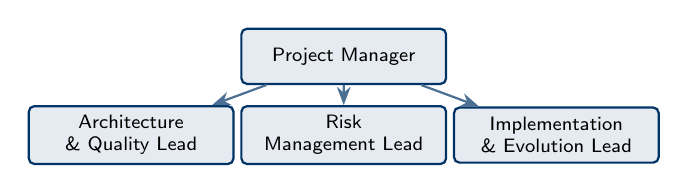
\begin{tikzpicture}[
  every node/.style={rectangle, rounded corners=2pt, draw=udblue, fill=udblue!10,
                     thick, minimum width=2.6cm, minimum height=0.7cm,
                     align=center, font=\scriptsize\sffamily},
  level distance=1.0cm, sibling distance=2.7cm,
  edge from parent/.style={draw=udblue!70, thick, -Stealth}]
\node {Project Manager}
  child {node {Architecture\\\& Quality Lead}}
  child {node {Risk\\Management Lead}}
  child {node {Implementation\\\& Evolution Lead}};
\end{tikzpicture}
\caption{CSAS team structure for Workshop No.\ 3.}
\label{fig:org}
\end{figure}

The responsibility matrix consolidating the role descriptions is presented
in Table~\ref{tab:resp}.

\begin{table}[H]
\centering
\caption{Responsibility matrix.}
\label{tab:resp}
\renewcommand{\arraystretch}{1.2}
\footnotesize
\begin{tabularx}{\columnwidth}{>{\bfseries}lX}
\toprule
\rowcolor{tableheader} Role & Main responsibilities \\
\midrule
Project Manager      & Planning, scheduling, coordination, control, integration of sections \\
Architecture Lead    & System design, quality framework, standards alignment \\
Risk Manager         & Risk identification, scoring, mitigation, contingency \\
Implementation Lead  & Implementation strategy, evolution summary, GitHub management \\
\bottomrule
\end{tabularx}
\end{table}

\subsection{Project Timeline and Critical Path}

The project is structured in six phases summing to twelve working days, with
the dependencies shown in Table~\ref{tab:timeline}.

\begin{table}[H]
\centering
\caption{Project phases, durations and dependencies.}
\label{tab:timeline}
\renewcommand{\arraystretch}{1.2}
\footnotesize
\begin{tabularx}{\columnwidth}{>{\bfseries}l X c l}
\toprule
\rowcolor{tableheader} Phase & Activity & Days & Depends on \\
\midrule
Planning         & Define objectives \& scope          & 2 & --- \\
Design           & Develop system architecture         & 3 & Planning \\
Analysis         & Perform risk assessment             & 2 & Design \\
Project planning & Develop schedule and plans          & 2 & Analysis \\
Integration      & Compile and unify document          & 2 & All phases \\
Delivery         & Final review and submission         & 1 & Integration \\
\bottomrule
\end{tabularx}
\end{table}

\subsubsection*{Milestones}
M1 Project Start; M2 Architecture Completed; M3 Risk Analysis Completed;
M4 Document Integration Completed; M5 Final Submission.

\subsubsection*{Critical Path}
\textbf{Planning $\rightarrow$ Design $\rightarrow$ Analysis $\rightarrow$
Project Planning $\rightarrow$ Integration $\rightarrow$ Delivery.} Any
slippage on these activities directly displaces the submission date; no
parallel float is available because each phase consumes outputs of the
previous one.

\subsubsection*{Gantt Chart}
The schedule is illustrated in Figure~\ref{fig:gantt}.

\begin{figure}[H]
\centering
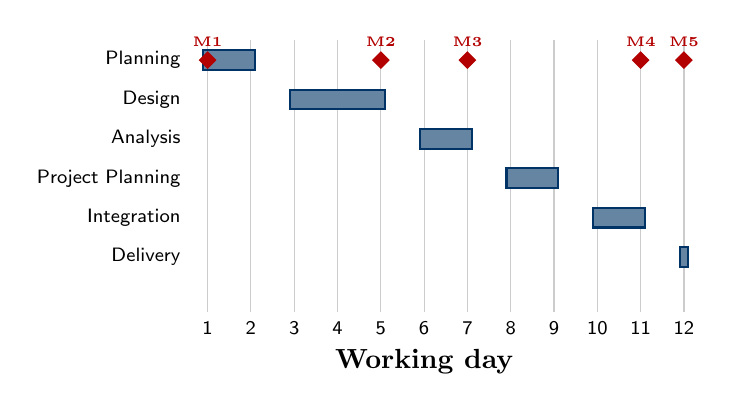
\begin{tikzpicture}[x=0.55cm, y=0.5cm, font=\scriptsize\sffamily]

% Day axis
\foreach \d in {1,...,12}
  \draw[gray!40] (\d,-0.4) -- (\d,6.5);
\foreach \d in {1,...,12}
  \node[anchor=north] at (\d,-0.4) {\d};
\node[anchor=north, font=\bfseries] at (6,-1.1) {Working day};

% Phase rows
\foreach \name/\start/\end/\row in {
  Planning/1/2/6,
  Design/3/5/5,
  Analysis/6/7/4,
  Project Planning/8/9/3,
  Integration/10/11/2,
  Delivery/12/12/1}{
    \node[anchor=east] at (0.6,\row) {\name};
    \fill[udblue!60, draw=udblue, thick]
      (\start-0.1,\row-0.25) rectangle (\end+0.1,\row+0.25);
}

% Milestones (diamonds)
\foreach \day/\label in {1/M1, 5/M2, 7/M3, 11/M4, 12/M5}{
  \node[diamond, draw=udred, fill=udred, inner sep=1.5pt] at (\day,6) {};
  \node[anchor=south, font=\tiny\bfseries, text=udred] at (\day,6.1) {\label};
}

\end{tikzpicture}
\caption{Project Gantt chart with the five milestones (M1--M5) anchored on
the critical path.}
\label{fig:gantt}
\end{figure}

\subsection{Resource Management Plan}

\begin{table}[H]
\centering
\caption{Resource management plan.}
\label{tab:resources}
\renewcommand{\arraystretch}{1.2}
\footnotesize
\begin{tabularx}{\columnwidth}{>{\bfseries}l X l}
\toprule
\rowcolor{tableheader} Resource type & Description & Responsible \\
\midrule
Human         & Four-member project team             & All members \\
Software      & \LaTeX, Word, draw.io, GitHub        & Team \\
Communication & WhatsApp, Google Meet                & PM \\
Time          & 12 working days (estimated)          & Project Manager \\
\bottomrule
\end{tabularx}
\end{table}

The Project Manager monitors resource utilization on a weekly basis and
escalates any deviation greater than 20\,\% from the plan to the team for
re-planning.

\subsection{Communication and Control Plan}

\textbf{Communication.} Primary channel: WhatsApp (asynchronous). Synchronous
meetings: Google Meet, twice per week, agenda sent 24~h in advance.
\textbf{Control.} Weekly progress reviews; partial submissions per role
checked by the PM against the deliverable index; final team validation
24~h before submission. \textbf{Escalation.} Any blocker open for more
than 24~h is escalated to the PM and, if unresolved, to the course
instructor.

% =============================================================================
\section{Implementation Strategy and Readiness Assessment}
\label{sec:implementation}

Although the workshop deliverable is a design and not a software product,
the implementation strategy is documented to demonstrate that the design is
\emph{implementation-ready}. The strategy adopts a phased deployment model,
defines infrastructure requirements, and integrates change management
procedures.

\subsection{Phased Deployment}

The deployment is organized in three phases (Figure~\ref{fig:phases}):

\begin{itemize}[leftmargin=*]
  \item \textbf{Phase 1 -- Pilot (4 weeks).} Restricted to a single faculty
  building and a closed user group of approximately 200 users. Exit
  criteria: all KPIs of Table~\ref{tab:metrics} met for two consecutive
  weeks and zero critical incidents.
  \item \textbf{Phase 2 -- Controlled rollout (8 weeks).} Extended to the
  full campus with feature flags enabling gradual exposure. Exit
  criteria: adoption rate $\geq$ 30\,\% of the target population and
  delivery success $\geq$ 99.5\,\% in real conditions.
  \item \textbf{Phase 3 -- Full operation (continuous).} The system is
  declared production-grade. Continuous improvement, security updates and
  capacity planning are governed by the change management procedure.
\end{itemize}

\begin{figure}[H]
\centering
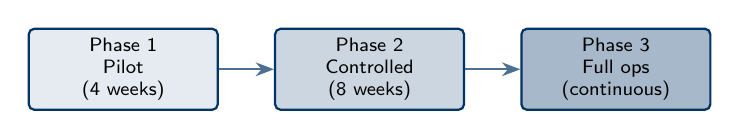
\begin{tikzpicture}[node distance=0.6cm and 0.7cm]
\node[process, fill=udblue!10] (p1) {Phase 1\\Pilot\\(4 weeks)};
\node[process, right=of p1, fill=udblue!20] (p2) {Phase 2\\Controlled\\(8 weeks)};
\node[process, right=of p2, fill=udblue!35] (p3) {Phase 3\\Full ops\\(continuous)};
\draw[arrow] (p1) -- (p2);
\draw[arrow] (p2) -- (p3);
\end{tikzpicture}
\caption{Phased deployment with explicit exit gates between phases.}
\label{fig:phases}
\end{figure}

\subsection{Technical Infrastructure Requirements}

\begin{itemize}[leftmargin=*]
  \item \textbf{Compute.} Kubernetes cluster of at least three worker
  nodes spread across two availability zones, with auto-scaling between
  3 and 12 nodes.
  \item \textbf{Storage.} PostgreSQL primary--standby (synchronous
  replication), Redis cache, object storage for evidence attachments.
  \item \textbf{Networking.} Public load balancer with TLS 1.3
  termination, private VPC for service-to-service traffic.
  \item \textbf{Observability.} Prometheus + Grafana for metrics, ELK
  stack for centralized logs, Jaeger for distributed traces.
  \item \textbf{External integrations.} Two SMS providers (active--active),
  FCM and APNs accounts, formal SLA with the local police communications
  unit.
\end{itemize}

\subsection{Change Management Procedure}

Every change goes through a four-step procedure: (i) request and impact
analysis, (ii) approval by the change advisory board (PM +
Architecture Lead + Risk Manager), (iii) scheduled deployment with a
rollback plan, and (iv) post-deployment review. Emergency changes follow
an expedited path with mandatory retrospective within 48\,h.

\subsection{Training and User Adoption}

The adoption strategy combines (a) a 30-minute on-boarding session for
faculty and staff multipliers, (b) a 2-minute self-guided in-app tutorial
for end users, (c) printed quick-reference cards distributed in
high-traffic areas of the campus, and (d) a feedback channel inside the
app routed to the Implementation Lead.

\subsection{Readiness Assessment}

The system is considered ready for Phase 1 when the following readiness
indicators are simultaneously satisfied: architecture sign-off by the
Architecture Lead; risk register reviewed and accepted by the Risk Manager
with no open critical risks; security scan clean; load test passed at
300\,\% projected traffic; backup/restore drill executed within the last
30 days; UAT scenarios green for the pilot user group; on-call rotation
defined and documented. Failure of any indicator delays the pilot start.

% =============================================================================
\section{Evolution and Continuous Improvement}
\label{sec:evolution}

This section documents how the design has matured through the
analysis--design--refinement cycle of Workshops 1, 2 and 3, and establishes
the mechanisms that will keep the system evolving after deployment.

\subsection{From Workshop No.\ 1 to Workshop No.\ 2}

Workshop No.\ 1 surfaced three findings that shaped the architecture of
Workshop No.\ 2: (i) reporting friction is the primary adoption barrier;
(ii) authority response time is the dominant component of perceived
latency; and (iii) connectivity is highly heterogeneous across the
campus~\cite{csas_w1}. Workshop No.\ 2 responded with, respectively, a
mobile-first interface limited to three interactions, an asynchronous
event-driven backbone that absorbs authority-side delays, and an SMS/USSD
fallback~\cite{csas_w2}.

\subsection{From Workshop No.\ 2 to Workshop No.\ 3}

Workshop No.\ 3 strengthens the previous design along four explicit
vectors:

\begin{itemize}[leftmargin=*]
  \item \textbf{Quality formalization.} Quality attributes that were
  qualitatively claimed in Workshop No.\ 2 are now bound to measurable
  KPIs (Table~\ref{tab:metrics}) and to recognized standards
  (Table~\ref{tab:standards}).
  \item \textbf{Risk explicitness.} Risks that were implicit in the
  Workshop No.\ 2 architecture (overload, breach, false reports) are now
  registered, scored, mitigated and monitored
  (Table~\ref{tab:risks}, Figure~\ref{fig:heatmap}).
  \item \textbf{Project executability.} The team structure, schedule and
  communication plan transform the design into an executable project
  (Section~\ref{sec:pm}).
  \item \textbf{Implementation readiness.} A phased deployment with
  explicit exit gates and a readiness assessment makes the path to
  production observable and auditable
  (Section~\ref{sec:implementation}).
\end{itemize}

\subsection{Comparative Summary}

\begin{table}[H]
\centering
\caption{Workshop-to-workshop evolution of key dimensions.}
\label{tab:evolution}
\renewcommand{\arraystretch}{1.2}
\footnotesize
\begin{tabularx}{\columnwidth}{>{\bfseries}l X X X}
\toprule
\rowcolor{tableheader} Dimension & Workshop 1 & Workshop 2 & Workshop 3 \\
\midrule
Focus           & Analysis        & Design          & Robustness \& mgmt. \\
Quality attr.\  & Implicit        & Stated          & Measured \& mapped \\
Risks           & Identified      & Partly addressed& Registered \& mitigated \\
Standards       & Mentioned       & Referenced      & Mapped to components \\
Project mgmt.   & ---             & Lightweight     & PMBOK-aligned plan \\
\bottomrule
\end{tabularx}
\end{table}

\subsection{Continuous Improvement Mechanisms}

Post-deployment, four mechanisms keep the system evolving:

\begin{enumerate}[leftmargin=*]
  \item \emph{User feedback loop} via in-app channel, triaged weekly by
  the Implementation Lead.
  \item \emph{Monthly KPI review} where the seven metrics of
  Table~\ref{tab:metrics} are evaluated; any sustained deviation triggers
  a corrective-action ticket.
  \item \emph{Quarterly risk re-assessment} updating the register with
  new threats and retiring closed ones.
  \item \emph{Annual architecture review} aligned with ISO~9001
  management-review requirements, producing a formal report and an
  updated roadmap.
\end{enumerate}

\subsection{Success Metrics}

Three composite indicators measure post-implementation effectiveness:
(i) \emph{Operational health} = average of latency, uptime and delivery
success against their targets; (ii) \emph{User health} = adoption and
usability scores; (iii) \emph{Compliance health} = ratio of clean
quarterly audits. The system is deemed successful when all three
composites remain above 0.85 for two consecutive quarters.

% =============================================================================
\section{Ethical and Legal Considerations}
\label{sec:ethics}

Because CSAS handles location data, security incidents and personal
identifiers, ethical and legal considerations are first-class design
constraints rather than after-the-fact compliance checks.

\subsection{Data Protection}

The system complies with Ley~1581 de 2012 (Régimen General de Protección
de Datos Personales) of the Republic of Colombia and its regulatory
decree~\cite{ley1581}. Personal data is collected only with explicit,
informed consent obtained at on-boarding; data is encrypted in transit
(TLS 1.3) and at rest (AES-256); access is governed by role-based
controls and audited; users can request deletion of their data at any
time through a dedicated endpoint.

\subsection{Minimization and Purpose Binding}

Only the data strictly necessary to verify and disseminate an alert is
retained: incident type, geolocation truncated to a configurable
precision, timestamp and an anonymous reporter ID. Detailed identity
information is not stored alongside reports; it is queried just-in-time
for verification when strictly required.

\subsection{Avoidance of Harm}

The verification engine and the user reputation score are designed to
\emph{minimize false alerts} that could induce panic, but never to
suppress genuine reports. A human-in-the-loop review is required before
alerts of the highest severity are propagated to authorities, balancing
speed against the risk of weaponizing the system against innocent
parties.

\subsection{Equity of Access}

The SMS/USSD fallback and the Spanish-first, low-literacy interface
prevent the system from becoming a privilege of users with high-end
smartphones or stable connectivity, addressing an equity concern that
emerged from the Workshop No.\ 1 fieldwork.

\subsection{Transparency and Accountability}

Privacy policies, the data-retention schedule and the algorithmic
verification heuristics are documented publicly. Every automated action
that affects a user (e.g., report rejection, reputation downgrade) is
logged and appealable through an explicit channel.

% =============================================================================
\section{Repository Management}
\label{sec:repo}

All Workshop No.\ 3 artefacts are stored in the
\texttt{Workshop\_3\_Management} folder of the course GitHub repository,
following the structure already established for Workshops 1 and 2. The
folder contains:

\begin{itemize}[leftmargin=*]
  \item \texttt{docs/} --- this PDF and its \LaTeX{} sources.
  \item \texttt{diagrams/} --- editable \texttt{drawio} and
  \texttt{tikz} sources of all figures.
  \item \texttt{risk\_register/} --- spreadsheet export of
  Table~\ref{tab:risks} for tooling interoperability.
  \item \texttt{pm/} --- Gantt source, communication matrix, role
  descriptions.
  \item \texttt{README.md} --- updated to cover all three workshops with
  a navigation index and a summary of the evolution
  (Section~\ref{sec:evolution}).
\end{itemize}

The \texttt{main} branch is protected; every change reaches it through a
pull request reviewed by at least one team member other than the author,
mirroring the CI/CD discipline that the production system will apply.

% =============================================================================
\section{Conclusion}
\label{sec:conclusion}

Workshop No.\ 3 closes the analysis--design--refinement cycle of the CSAS
project by transforming the architectural blueprint of Workshop No.\ 2
into a robust, risk-aware and project-managed solution that is ready for
implementation. The architecture has been re-justified component by
component against ISO/IEC~25010 quality attributes and IEEE/CMMI/ISO
standards; ten risks have been formally registered, scored, and matched
with mitigation, contingency and monitoring strategies; a project
management plan articulates roles, schedule, resources and communications
along the critical path; a phased deployment with explicit readiness
indicators establishes the path to production; and a continuous-improvement
mechanism guarantees that the system will keep evolving with its users.

The most significant lesson from this workshop is that \emph{robustness
is not a property added at the end of the design}: it is the product of
explicitly binding every architectural decision to a measurable quality
attribute and to a foreseeable risk. By the end of this workshop, every
component of CSAS has both bindings, and the design is therefore not only
viable but auditable, sustainable and improvable.

% =============================================================================
\begin{thebibliography}{99}

\bibitem{csas_w1}
Garzon Herrera, F.~J., Quintero Gordillo, J.~E., Garrido Medina, H.~S., and
Cusba Marin, G.~M.,
\emph{Workshop No.\ 1: Systems Analysis of the Community Security Alert
System (CSAS)}, Universidad Distrital Francisco José de Caldas, 2026.

\bibitem{csas_w2}
Garzon Herrera, F.~J., Quintero Gordillo, J.~E., Garrido Medina, H.~S., and
Cusba Marin, G.~M.,
\emph{Workshop No.\ 2: System Design of the Community Security Alert
System (CSAS)}, Universidad Distrital Francisco José de Caldas, 2026.

\bibitem{iso9001}
International Organization for Standardization,
\emph{ISO 9001:2015 --- Quality management systems --- Requirements},
ISO, Geneva, 2015.

\bibitem{iso25010}
International Organization for Standardization / IEC,
\emph{ISO/IEC 25010:2011 --- Systems and software engineering ---
SQuaRE --- System and software quality models}, 2011.

\bibitem{iso31000}
International Organization for Standardization,
\emph{ISO 31000:2018 --- Risk management --- Guidelines},
ISO, Geneva, 2018.

\bibitem{ieee830}
IEEE, \emph{IEEE Std 830-1998 --- Recommended Practice for Software
Requirements Specifications}, 1998.

\bibitem{ieee1633}
IEEE, \emph{IEEE Std 1633-2016 --- Recommended Practice on Software
Reliability}, 2016.

\bibitem{ieee12207}
IEEE / ISO / IEC, \emph{ISO/IEC/IEEE 12207:2017 --- Systems and
software engineering --- Software life cycle processes}, 2017.

\bibitem{cmmi}
CMMI Institute, \emph{CMMI for Development, Version 2.0}, ISACA, 2018.

\bibitem{pmbok}
Project Management Institute, \emph{A Guide to the Project Management
Body of Knowledge (PMBOK Guide)}, 7th ed., PMI, 2021.

\bibitem{ley1581}
Congreso de la República de Colombia,
\emph{Ley Estatutaria 1581 de 2012 --- Régimen General de Protección
de Datos Personales}, 2012.

\end{thebibliography}

\end{document}
